\documentclass[border=4pt]{standalone}
\usepackage{tikz}
\usepackage{pgfplots}
\pgfplotsset{compat=1.18}
\usetikzlibrary{shapes.geometric,arrows.meta,positioning,calc,fit,decorations.pathreplacing,backgrounds}
\definecolor{boxblue}{RGB}{225,238,252}
\definecolor{boxgreen}{RGB}{225,247,231}
\definecolor{boxorange}{RGB}{253,236,216}
\definecolor{boxgray}{RGB}{237,237,237}
\definecolor{boxred}{RGB}{253,226,226}
\begin{document}
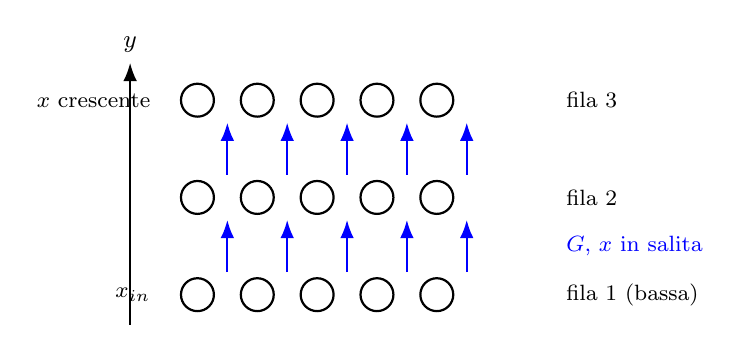
\begin{tikzpicture}[scale=0.95]
\foreach \y/\lab in {0/{fila 1 (bassa)}, 1.3/{fila 2}, 2.6/{fila 3}}{
  \foreach \x in {0,0.8,...,4.0}{
    \draw[thick] ({\x},{\y}) circle (0.22);
  }
  \node[font=\footnotesize,anchor=west] at (4.8,\y) {\lab};
}
% rising bubbles / flow arrows
\foreach \x in {0.4,1.2,2.0,2.8,3.6}{
  \draw[-{Latex},blue,thick] ({\x},{0.3}) -- ({\x},{1.0});
  \draw[-{Latex},blue,thick] ({\x},{1.6}) -- ({\x},{2.3});
}
\node[font=\footnotesize,blue,anchor=west] at (4.8,0.65) {$G$, $x$ in salita};
\node[font=\footnotesize,anchor=east] at (-0.5,0) {$x_{in}$};
\node[font=\footnotesize,anchor=east] at (-0.5,2.6) {$x$ crescente};
\draw[-{Latex},thick] (-0.9,-0.4) -- (-0.9,3.1) node[above,font=\small]{$y$};
\end{tikzpicture}
\end{document}
